\section*{Đề thi thử THPTQG Sở GD \& ĐT 25--26, Lần 1}

\caulc
\Opensolutionfile{ans}[ans/ans-26-2--SoGD-L1-LC]
%TN1-01
\begin{ex} %[Thi thử THPT, Nguyễn Văn Trỗi - Hà Tĩnh, 2025 - 2026] %[2H2N1-1]
	Cho hình hộp chữ nhật $ABCD.A'B'C'D'$. Khi đó, véc-tơ bằng véc-tơ $\vec{AB}$ là véc-tơ nào dưới đây?
	\choice
	{\True $\vec{D'C'}$}
	{$\vec{CD}$}
	{$\vec{BA}$}
	{$\vec{B'A'}$}
	\loigiai{
		\begin{center}
			\begin{tikzpicture}[line join = round, line cap = round, thick, scale = 0.7]
				\coordinate (vtv) at (-0.625, 2.25);
				\coordinate (A) at (0, 0);
				\coordinate (B) at (-1.2, -1.5);
				\coordinate (D) at (4, 0);
				\coordinate (C) at ($(B) + (D) - (A)$);
				\foreach \x in {A, B, C, D}
				\coordinate (\x') at ($(\x) + (vtv)$);
				\draw (B)--(C) (C)--(D) (B)--(B') (C)--(C') (D)--(D')
				(A')--(B') (B')--(C') (C')--(D') (D')--(A');
				\draw[dashed, thin](A)--(B) (A)--(D) (A)--(A');
				\foreach \i/\g in {A'/90, A/180, B/180, C/0, D/0, B'/180, D'/0, C'/0}
				{\draw[fill = black] (\i)circle(1.5pt) ($(\i)+(\g:3mm)$)node[scale = 0.7]{$\i$};}
			\end{tikzpicture}
		\end{center}
		Ta có: $\vec{AB} = \vec{DC} = \vec{D'C'}$.
	}
\end{ex}

%TN1-02
\begin{ex} %[Thi thử THPT, Nguyễn Văn Trỗi - Hà Tĩnh, 2025 - 2026] %[2D1N4-1]
	Đường tiệm cận ngang của đồ thị hàm số $y = \dfrac{3x - 2}{x + 1}$ là
	\choice
	{\True $y = 3$}
	{$y = 1$}
	{$x = -1$}
	{$y = -2$}
	\loigiai{
		Ta có: $\heva{
			& \mathop{\lim}\limits_{x \to +\infty}{\dfrac{3x - 2}{x + 1}} = 3 \\
			& \mathop{\lim}\limits_{x \to -\infty}{\dfrac{3x - 2}{x + 1}} = 3} \Rightarrow y = 3$ là đường tiệm cận ngang của đồ thị hàm số.
	}
\end{ex}

%TN1-03
\begin{ex} %[Thi thử THPT, Nguyễn Văn Trỗi - Hà Tĩnh, 2025 - 2026] %[2D4N1-4]
	Họ nguyên hàm của hàm số $f\left(x\right) = {\mathrm{e}}^x + 2x$ là
	\choice
	{$\dfrac{{\mathrm{e}}^{x + 1}}{x + 1} + x^2 + C$}
	{${\mathrm{e}}^x + 2 + C$}
	{\True ${\mathrm{e}}^x + x^2 + C$}
	{${\mathrm{e}}^x + 2x^2 + C$}
	\loigiai{
		Ta có: $\displaystyle\int{\left({\mathrm{e}}^x + 2x\right)}{\mathrm{\, d}}x = {\mathrm{e}}^x + x^2 + C$.
	}
\end{ex}

%TN1-04
\begin{ex} %[Thi thử THPT, Nguyễn Văn Trỗi - Hà Tĩnh, 2025 - 2026] %[2H5N1-3]
	Trong không gian $Oxyz$, mặt phẳng đi qua $A\left(1; -2; 3\right)$ và có véc-tơ pháp tuyến $\vec n = \left(2; 1; -1\right)$ có phương trình là
	\choice
	{\True $2x + y - z + 3 = 0$}
	{$x - 2y + 3z + 3 = 0$}
	{$2x + y - z = 0$}
	{$2x + y - z - 3 = 0$}
	\loigiai{
		Mặt phẳng đi qua $A\left(1; -2; 3\right)$ và có véc-tơ pháp tuyến $\vec n = \left(2; 1; -1\right)$ có phương trình là $$2\left(x - 1\right) + \left(y + 2\right) - \left(z - 3\right) \Leftrightarrow 2x + y - z + 3 - 0.$$
	}
\end{ex}

%TN1-05
\begin{ex} %[Thi thử THPT, Nguyễn Văn Trỗi - Hà Tĩnh, 2025 - 2026] %[2D4N3-1]
	Diện tích hình phẳng giới hạn bởi đồ thị $y = x^2 - 4x$, trục $Ox$, $x = 0$, $x = 4$ được tính bằng
	\choice
	{$\displaystyle\int\limits_0^4{\left(x^2 - 4x\right)}{\mathrm{\, d}}x$}
	{$\displaystyle\int\limits_0^4{\left(x^2 - 4x\right)^2}{\mathrm{\, d}}x$}
	{\True $\displaystyle\int\limits_0^4{\left|x^2 - 4x\right|}{\mathrm{\, d}}x$}
	{$\pi\displaystyle\int\limits_0^4{\left(x^2 - 4x\right)^2}{\mathrm{\, d}}x$}
	\loigiai{
		Diện tích hình phẳng giới hạn bởi đồ thị $y = x^2 - 4x$, trục $Ox$, $x = 0$, $x = 4$ được tính bằng $\displaystyle\int\limits_0^4{\left|x^2 - 4x\right|}{\mathrm{\, d}}x$.
	}
\end{ex}

%TN1-06
\begin{ex} %[Thi thử THPT, Nguyễn Văn Trỗi - Hà Tĩnh, 2025 - 2026] %[1H8N2-2]
	Cho lăng trụ đứng tam giác $ABC.A'B'C'$. Đường thẳng $AA'$ vuông góc với mặt phẳng nào dưới đây?
	\choice
	{$\left(AB'C'\right)$}
	{$\left(ABB'A'\right)$}
	{\True $\left(ABC\right)$}
	{$\left(BCC'B'\right)$}
	\loigiai{
		\begin{center}
			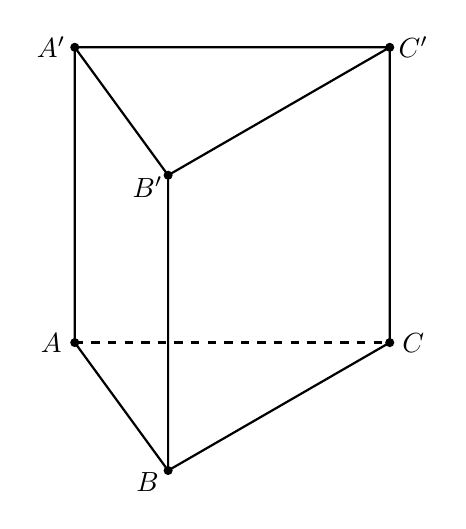
\begin{tikzpicture}
				\path 
				(0:0) coordinate (A)
				++(0:4) coordinate (C)
				++(-150:3.25) coordinate (B);
				\foreach \x in {A, B, C}
				\draw (\x)++(90:3.75) coordinate (\x');
				\draw[thick] (A)--(B) (B)--(C) (A)--(A') (B)--(B') (C)--(C')
				(A')--(B') (B')--(C') (C')--(A');
				\draw[dashed, thick] (A)--(C);
				\foreach \x/\g in {A/180, B/-150, C/0, A'/180, B'/-150, C'/0}
				\draw[fill = black] (\x)circle(.05)+(\g:3mm)node{$\x$};
			\end{tikzpicture}
		\end{center}
		Do $ABC.A'B'C'$ là lăng trụ đứng nên $AA' \perp \left(ABC\right)$.
	}
\end{ex}

%TN1-07
\begin{ex} %[Thi thử THPT, Nguyễn Văn Trỗi - Hà Tĩnh, 2025 - 2026] %[2H5N2-2]
	Trong không gian $Oxyz$, đường thẳng $d \colon \dfrac{x - 2}{-1} = \dfrac{y + 1}{3} = \dfrac{z}{2}$ có một véc-tơ chỉ phương là
	\choice
	{$\vec u = \left(1; -3; 2\right)$}
	{\True $\vec u = \left(-1; 3; 2\right)$}
	{$\vec u = \left(2; -1; 0\right)$}
	{$\vec u = \left(1; 3; -2\right)$}
	\loigiai{
		Đường thẳng $d \colon \dfrac{x - 2}{-1} = \dfrac{y + 1}{3} = \dfrac{z}{2}$ có một véc-tơ chỉ phương là $\vec u = \left(-1; 3; 2\right)$.
	}
\end{ex}

%TN1-08
\begin{ex} %[Thi thử THPT, Nguyễn Văn Trỗi - Hà Tĩnh, 2025 - 2026] %[1D6N4-2]
	Nghiệm của phương trình $\log_2\left(x - 1\right) = 3$ là
	\choice
	{$x = 8$}
	{\True $x = 9$}
	{$x = 10$}
	{$x = 7$}
	\loigiai{
		Ta có: $\log_2\left(x - 1\right) = 3 \Leftrightarrow \heva{
			& x - 1 > 0 \\
			& x - 1 = 2^3} \Leftrightarrow \heva{
			& x > 1 \\
			& x = 9} \Leftrightarrow x = 9$.
	}
\end{ex}

%TN1-09
\begin{ex} %[Thi thử THPT, Nguyễn Văn Trỗi - Hà Tĩnh, 2025 - 2026] %[1D1N5-3]
	Nghiệm của phương trình $\cos x = 1$ là
	\choice
	{$x = \dfrac{\pi}{2} + k\pi$}
	{$x = k\pi$}
	{$x = \pi + k2\pi$}
	{\True $x = k2\pi$}
	\loigiai{
		Ta có: $\cos x = 1 \Leftrightarrow x = k2\pi$.
	}
\end{ex}

%TN1-10
\begin{ex} %[Thi thử THPT, Nguyễn Văn Trỗi - Hà Tĩnh, 2025 - 2026] %[2D1H1-1]
	Hàm số $y = x^3 - 3x$ nghịch biến trên khoảng nào?
	\choice
	{$\left(-\infty; -1\right)$}
	{$\left(0; +\infty\right)$}
	{$\left(-\infty; +\infty\right)$}
	{\True $\left(-1; 1\right)$}
	\loigiai{
		Đạo hàm: $y' = 3x^2 - 3 = 0 \Leftrightarrow x = \pm 1$. \\
		Bảng xét dấu đạo hàm:
		\begin{center}
			
\begin{tikzpicture}[>= stealth]
				\tkzTabInit[nocadre = false, lgt = 1.25, espcl = 2.75, deltacl = 0.6]
				{$x$ /0.75, $y'$ /0.75}
				{$-\infty$, $-1$, $1$, $+\infty$}
				\tkzTabLine{, +, z, -, z, +,}
			\end{tikzpicture}
		\end{center}
		Vậy hàm số nghịch biến trên khoảng $\left(-1; 1\right)$.
	}
\end{ex}

%TN1-11
\begin{ex} %[Thi thử THPT, Nguyễn Văn Trỗi - Hà Tĩnh, 2025 - 2026] %[1D2N2-4]
	Cho cấp số cộng $\left(u_n\right)$ có $u_1 = -2$ và công sai $d = 4$. Giá trị của $u_4$ bằng
	\choice
	{$6$}
	{$14$}
	{\True $10$}
	{$6$}
	\loigiai{
		Ta có: $u_4 = u_1 + 3d = -2 + 3 \cdot 4 = 10$.
	}
\end{ex}

%TN1-12
\begin{ex} %[Thi thử THPT, Nguyễn Văn Trỗi - Hà Tĩnh, 2025 - 2026] %[1D5N2-2]
	Doanh thu bán hàng trong $20$ ngày được lựa chọn ngẫu nhiên của một cửa hàng được ghi lại ở bảng sau (đơn vị: triệu đồng).
	\begin{center}
		\begin{tabular}{|c|c|c|c|c|c|}
			\hline
			Doanh thu & $\left[5; 7\right)$ & $\left[7; 9\right)$ & $\left[9; 11\right)$ & $\left[11; 13\right)$ & $\left[13; 15\right)$ \\
			\hline
			Số ngày & $2$ & $7$ & $7$ & $3$ & $1$ \\
			\hline
		\end{tabular}
	\end{center}
	Trung vị của mẫu số liệu trên thuộc khoảng nào trong các khoảng dưới đây?
	\choice
	{$\left[7; 9\right)$}
	{$\left[11; 13\right)$}
	{\True $\left[9; 11\right)$}
	{$\left[13; 15\right)$}
	\loigiai{
		Cỡ mẫu là $n = 20 \Rightarrow \dfrac{n}{2} = 10$ nên nhóm chứa trung vị là $\left[9; 11\right)$.
	}
\end{ex}
\Closesolutionfile{ans}


\cauds
\Opensolutionfile{ans}[ans/ans-26-2--SoGD-L1-DS]
%TN2-01
\begin{ex} %[Thi thử THPT, Nguyễn Văn Trỗi - Hà Tĩnh, 2025 - 2026] %[2D1V1-5]
	Một công ty công nghệ phát hành một video quảng cáo trên mạng xã hội. Số lượng người xem tích lũy $P\left(t\right)$ (đơn vị: người) sau thời gian $t$ (đơn vị: ngày) được mô hình hóa bởi hàm số: $$P\left(t\right) = \dfrac{100000}{1 + 999{\mathrm{e}}^{-0{,}5t}}.$$ Số lượng người xem tối đa dự kiến trong tệp khách hàng tiềm năng là $100000$ người. Tốc độ lan truyền video tại thời điểm $t$ được xác định bởi hàm số $P'\left(t\right)$.	
	\choiceTF[1]
	{\True Tại thời điểm bắt đầu phát hành video $\left(t = 0\right)$, đã có $100$ người xem video này}
	{Để đạt được $90\%$ số lượng người xem mục tiêu (tương ứng $90000$ người), công ty cần khoảng $18$ ngày (làm tròn đến hàng đơn vị)}
	{Sau $10$ ngày kể từ khi phát hành, tổng số lượng người xem video đạt hơn $15000$ người}
	{\True Tại thời điểm $t = 5$, tốc độ lan truyền của video vẫn đang trên đà tăng}
	\loigiai{
		\begin{itemchoice}
			\itemch $P\left(0\right) = \dfrac{100000}{1 + 999{\mathrm{e}}^{-0{,}5 \cdot 0}} = 100$ (người).
			\itemch $P\left(t\right) = \dfrac{100000}{1 + 999{\mathrm{e}}^{-0{,}5t}} = 90000 \Leftrightarrow 1 + 999{\mathrm{e}}^{-0{,}5t} = \dfrac{10}{9} \Leftrightarrow t = -2\ln\left(\dfrac{\dfrac{10}{9} - 1}{999}\right) \approx 18{,}2080$. \\
			Vậy cần khoảng $19$ ngày để đạt được $90\%$ số lượng người xem mục tiêu.
			\itemch $P\left(10\right) = \dfrac{100000}{1 + 999{\mathrm{e}}^{-0{,}5 \cdot 10}} \approx 12935$ (người).
			\itemch	$P'\left(t\right) = -\dfrac{100000\left(1 + 999{\mathrm{e}}^{-0{,}5t}\right)'}{\left(1 + 999{\mathrm{e}}^{-0{,}5t}\right)^2} = \dfrac{100000 \cdot 999 \cdot 0{,}5{\mathrm{e}^{-0{,5}t}}}{\left(1 + 999{\mathrm{e}}^{-0{,}5t}\right)^2}$. \\
			Kiểm tra $P''\left(5\right) \approx 290{,}3955 > 0$ nên tốc độ lan truyền tại thời điểm $t = 5$ trên đà tăng.
		\end{itemchoice}
	}
\end{ex}

%TN2-02
\begin{ex} %[Thi thử THPT, Nguyễn Văn Trỗi - Hà Tĩnh, 2025 - 2026] %[2D1H5-1]
	Cho hàm số $y = f\left(x\right) = \dfrac{x^2 - x + 2}{x - 2}$ có đồ thị $\left(C\right)$.
	\choiceTF[1]
	{Hàm số đồng biến trên mỗi khoảng $\left(-\infty; 0\right)$ và $\left(2; +\infty\right)$}
	{\True Tập xác định của hàm số là $\mathscr{D} = \mathbb{R} \setminus \left\{2\right\}$}
	{\True Đường thẳng $y = x + 1$ là tiệm cận xiên của đồ thị $\left(C\right)$}
	{Đồ thị $\left(C\right)$ đi qua điểm $M\left(0; 2\right)$}
	\loigiai{
		\begin{itemchoice}
			\itemch Đạo hàm: $f'\left(x\right) = \dfrac{x^2 - 4x}{\left(x - 2\right)^2} = 0 \Leftrightarrow \hoac{
				& x = 0 \\
				& x = 4}$. \\
			Bảng xét dấu đạo hàm:
			\begin{center}
				
\begin{tikzpicture}[>= stealth]
					\tkzTabInit[nocadre = false, lgt = 1.25, espcl = 2.75, deltacl = 0.6]
					{$x$ /0.75, $f'\left(x\right)$ /0.75}
					{$-\infty$, $0$, $2$, $4$, $+\infty$}
					\tkzTabLine{, +, z, -, d, -, z, +,}
				\end{tikzpicture}
			\end{center}
			Vậy hàm số đồng biến trên các khoảng $\left(-\infty; 0\right)$ và $\left(4; +\infty\right)$.
			\itemch Tập xác định của hàm số là $\mathscr{D} = \mathbb{R} \setminus \left\{2\right\}$.		
			\itemch $f\left(x\right) = \dfrac{x^2 - x + 2}{x - 2} = x + 1 + \dfrac{4}{x - 2} \Rightarrow y = x + 1$ là tiệm cận xiên của đồ thị $\left(C\right)$.
			\itemch	Với $x = 0 \Rightarrow f\left(0\right) = -1$. Do đó, đồ thị $\left(C\right)$ không đi qua điểm $M\left(0; 2\right)$.
		\end{itemchoice}
	}
\end{ex}

%TN2-03
\begin{ex} %[Thi thử THPT, Nguyễn Văn Trỗi - Hà Tĩnh, 2025 - 2026] %[2H5V3-4]
	Trong một dự án khảo sát địa chất thăm dò tài nguyên, các nhà khoa học phát hiện một túi khí tự nhiên trong lòng đất được xác định có dạng hình cầu $\left(S\right)$, một lớp đá móng ngăn cách các địa tầng $\left(P\right)$. Với hệ trục $Oxyz$ phù hợp, đơn vị trên mỗi trục là chục mét. Mặt cầu $\left(S\right)$ có phương trình $\left(x - 2\right)^2 + \left(y - 3\right)^2 + \left(z + 7\right)^2 = 16$. Lớp đá móng là mặt phẳng $\left(P\right)$ có phương trình $x + y + z - 15 = 0$. Để thực hiện việc khai thác, các nhà khoa học đặt mũi khoan được định hướng bắt đầu từ vị trí $A\left(1; 2; 1\right)$ và tiến tới liên tục theo phương của vectơ $\vec u = \left(1; 1; -8\right)$. Ngoài ra, một trạm quan trắc địa chấn được đặt cố định tại vị trí $K\left(2; 3; 5\right)$ để theo dõi các biến động cơ học trong quá trình khoan.
	\begin{center}
		\begin{tikzpicture}[scale = .5]
			\def\r{4}
			\foreach \x/\i/\g in {x/-150/12, y/0/15, z/90/8}
			\draw[->, thick] (0:0)--++(\i:\g)node[above left]{$\x$};
			\path
			(2, 1) coordinate (A)node[above left]{$A$}
			(3, 5) coordinate (K)node[above	left]{$K$}
			(3, -7) coordinate (I)
			++(0:\r) coordinate (M)
			($(A)!2/3!(I)$) coordinate (N);
			\draw[dashed] (M) arc (0:180:{\r} and {\r/3});
			\draw[thick] (I) circle (\r)
			(M) arc (360:180:{\r} and {\r/3});
			\shade[ball color = cyan!60, opacity = 0.7] (I) circle (\r);
			\fill[orange!15, opacity = .7] (-8, -5)--(10, 0)--(20, -8)--(2, -13)--cycle;
			\filldraw (I) circle (2pt) node[right]{$I$};
			\draw[->, dashed, thick, red] (A)--(N)node[pos = .5, right, gray]{\scriptsize Hướng mũi khoan};
			\fill[black] (A) circle (3pt) 
			(K) circle (3pt) node[right]{Trạm quan trắc}
			(20, -8) node[left, xshift = -24pt, yshift = 6pt, gray]{\scriptsize Lớp đá móng};
		\end{tikzpicture}
	\end{center}
	\choiceTF[1]
	{Túi khí $\left(S\right)$ bị lớp đá móng $\left(P\right)$ chia thành hai phần có thể tích bằng nhau}
	{\True Quỹ đạo của mũi khoan được mô tả bởi một phần đường thẳng $d$ có phương trình chính tắc là $\dfrac{x - 1}{1} = \dfrac{y - 2}{1} = \dfrac{z - 1}{-8}$}
	{\True Trên quỹ đạo chuyển động của mình, mũi khoan sẽ đi xuyên qua túi khí $\left(S\right)$ tạo thành một đoạn đường ống trong lòng túi khí có độ dài là $80$ m}
	{Khi mũi khoan bắt đầu chạm vào túi khí $\left(S\right)$ thì tín hiệu địa chấn nhận được là mạnh nhất. Khi đó khoảng cách từ trạm quan trắc đến điểm nhận được tín hiệu mạnh nhất bằng $79$ m (kết quả làm tròn đến hàng đơn vị)}
	\loigiai{
		\begin{itemchoice}
			\itemch Nếu $\left(P\right)$ chia $\left(S\right)$ thành hai phần có thể tích bằng nhau thì $I \in \left(P\right)$. \\
			Ta thấy $2 + 3 - 7 - 15 = -17 \ne 0 \Rightarrow I \notin \left(P\right)$.
			\itemch Đường thẳng $d$ đi qua điểm $A\left(1; 2; 1\right)$ và có một véc-tơ chỉ phương $\vec u = \left(1; 1; -8\right)$ nên có phương trình chính tắc là $d \colon \dfrac{x - 1}{1} = \dfrac{y - 2}{1} = \dfrac{z - 1}{-8}$.
			\itemch Ta có: $\vec{AI} = \left(1; 1; -8\right)$ nên $\vec u$ cùng phương với $\vec{AI}$. Khi đó, mũi khoan sẽ đi qua tâm $I$. \\
			Do đó, đoạn đường ống trong lòng túi khí có độ dài bằng đường kính của $\left(S\right)$, tức là $10 \cdot 2 \cdot 4 = 80$ (m).
			\itemch	Gọi $M$ là điểm chạm của mũi khoan vào túi khí. Khi đó, $M$ là giao điểm đầu tiên của đường thẳng $d \colon \heva{
				& x = 1 + t \\
				& y = 2 + t \\
				& z = 1 -8t}$ và $\left(S\right) \colon \left(x - 2\right)^2 + \left(y - 3\right)^2 + \left(z + 7\right)^2 = 16$. \\
			Ta có: $IM = R = 4$; $IA = \sqrt{\left(2 - 1\right)^2 + \left(3 - 2\right)^2 + \left(-7 - 1\right)^2} = \sqrt{66}$. \\
			Do đó, $\vec{IM} = \dfrac{4}{\sqrt{66}}\vec{IA} \Rightarrow \heva{
				& x_M - 2 = \dfrac{4}{\sqrt{66}} \cdot \left(-1\right) \\ 
				& y_M - 3 = \dfrac{4}{\sqrt{66}} \cdot \left(-1\right) \\
				& z_M + 7 = \dfrac{4}{\sqrt{66}} \cdot 8} \Leftrightarrow \heva{
				& x_M = \dfrac{66 - 2\sqrt{66}}{33} \\
				& y_M = \dfrac{99 - 2\sqrt{66}}{33} \\
				& z_M = \dfrac{-231 + 16\sqrt{66}}{33}}$. \\
			Vậy $10KM = 10\sqrt{\left(\dfrac{66 - 2\sqrt{66}}{33} - 2\right)^2 + \left(\dfrac{99 - 2\sqrt{66}}{33} - 3\right)^2 + \left(\dfrac{-231 + 16\sqrt{66}}{33} - 5\right)^2} \approx 81$ (m).
		\end{itemchoice}
	}
\end{ex}

%TN2-04
\begin{ex} %[Thi thử THPT, Nguyễn Văn Trỗi - Hà Tĩnh, 2025 - 2026] %[2D6V2-4]
	Một hệ thống y tế sử dụng AI để chẩn đoán bệnh dựa trên ảnh chụp X-quang. Biết tỉ lệ người mắc bệnh thực sự trong tập mẫu là $15\%$. Nếu một người có bệnh, AI nhận diện đúng với xác suất $90\%$. Nếu một người không có bệnh, AI nhận diện sai (báo có bệnh) với xác suất $5\%$.
	\choiceTF[1]
	{\True Xác suất AI chẩn đoán sai (âm tính giả hoặc dương tính giả) là $0{,}0575$}
	{\True Xác suất một người ngẫu nhiên được AI chẩn đoán là \lq\lq có bệnh\rq\rq bằng $0{,}1775$}
	{Để xác suất chẩn đoán đúng bệnh của AI lên tới $95\%$, cần nâng cấp hệ thống sao cho AI nhận diện đúng người có bệnh (độ nhạy) lên tối thiểu $99\%$}
	{\True Nếu AI chẩn đoán một người \lq\lq có bệnh\rq\rq, xác suất người đó thực sự mắc bệnh lớn hơn $0{,}75$}
	\loigiai{
		Gọi $A$ là biến cố \lq\lq Một người thực sự có bệnh\rq\rq; $B$ là biến cố \lq\lq AI chẩn đoán đúng\rq\rq; \\
		Khi đó, $\mathrm{P}\left(A\right) = 0{,}15$; $\mathrm{P}\left(\left.B\right|A\right) = 0{,}9$; $\mathrm{P}\left(\left.\overline{B}\right|\overline{A}\right) = 0{,}05$.
		\begin{itemchoice}
			\itemch Xác suất AI chẩn đoán sai là $$ \mathrm{P}\left(\overline{B}\right) = \mathrm{P}\left(A\right) \cdot \mathrm{P}\left(\left.\overline{B}\right|A\right) + \mathrm{P}\left(\overline{A}\right) \cdot \mathrm{P}\left(\left.\overline{B}\right|\overline{A}\right) = 0{,}15 \cdot \left(1 - 0{,}9\right) + \left(1 - 0{,}15\right) \times 0{,}05 = 0{,}0575.$$
			\itemch Xác suất một người được AI chẩn đoán \lq\lq có bệnh\rq\rq là $$\mathrm{P}\left(AB\right) + \mathrm{P}\left(\overline{A}\overline{B}\right) = \mathrm{P}\left(A\right) \cdot \mathrm{P}\left(\left.B\right|A\right) + \mathrm{P}\left(\overline{A}\right) \cdot \mathrm{P}\left(\left.\overline{B}\right|\overline{A}\right) = 0{,}15 \cdot 0{,}9 + \left(1 - 0{,}15\right) \cdot 0{,}05 = 0{,}1775.$$
			\itemch Gọi $x$ là khả năng AI nhận diện đúng người có bệnh sau khi nâng cấp. \\
			Xác suất AI chẩn đoán đúng là $$\mathrm{P}\left(B\right) = \mathrm{P}\left(A\right) \cdot \mathrm{P}\left(\left.B\right|A\right) + \mathrm{P}\left(\overline{A}\right) \cdot \mathrm{P}\left(\left.B\right|\overline{A}\right) = 0{,}15x + \left(1 - 0{,}15\right)\left(1 - 0{,}05\right) = 0{,}95 \Leftrightarrow x = 0{,}95.$$
			\itemch	Xác suất một người thực sự có bệnh, biết rằng AI chẩn đoán \lq\lq có bệnh\rq\rq là $$\dfrac{\mathrm{P}\left(AB\right)}{\mathrm{P}\left(AB\right) + \mathrm{P}\left(\overline{A}\overline{B}\right)} = \dfrac{0{,}15 \cdot 0{,}9}{0{,}1775} \approx 0{,}7606 > 0{,}75.$$
		\end{itemchoice}
	}
\end{ex}
\Closesolutionfile{ans}

\caukq
\Opensolutionfile{ans}[ans/ans-26-2--SoGD-L1-KQ]
%TN3-01
\begin{ex} %[Thi thử THPT, Nguyễn Văn Trỗi - Hà Tĩnh, 2025 - 2026] %[0D0V2-5]
	Có một cái túi đựng bốn thẻ, mỗi thẻ được ghi một số trong các số 1, 2, 3, 4 và hai cái hộp A, B. Hộp A chứa $8$ quả bóng trắng và $8$ quả bóng đen, hộp B rỗng. Bạn An thực hiện phép thử sau: lấy ngẫu nhiên một thẻ trong túi, kiểm tra số ghi trên thẻ rồi bỏ lại thẻ vào túi. Nếu số ghi trên thẻ là 1, lấy $1$ quả bóng trắng từ hộp A cho vào hộp B. Nếu số ghi trên thẻ là 2 hoặc 3, lấy $1$ quả bóng trắng và $1$ quả bóng đen từ hộp A cho vào hộp B. Nếu số ghi trên thẻ là 4, lấy $2$ quả bóng trắng và $1$ quả bóng đen từ hộp A cho vào hộp B. Sau khi thực hiện phép thử trên $4$ lần, khi số bóng trong hộp B là $8$ thì xác suất để có $2$ quả bóng đen trong hộp B	bằng $\dfrac{a}{b}$ ($a, b$ nguyên và $\dfrac{a}{b}$ tối giản). Khi đó $a + b$ bằng bao nhiêu?
	\shortans{$38$}
	\loigiai{
		Để hộp B có $8$ quả bóng sau $4$ lần bốc có các trường hợp sau.
		\begin{itemize}
			\item \textbf{Trường hợp 1:} Bốc $1$ thẻ số 1, $2$ thẻ số 2 hoặc 3 và $1$ thẻ số 4. \\
			Chọn $1$ lần bốc thẻ số 1, $1$ lần bốc thẻ số 4 và $2$ lần còn lại bốc thẻ số 2 hoặc 3: ${\mathrm{C}_4^1}{\mathrm{C}_3^1} \cdot 2 \cdot 2 = 48$ (cách).
			\item \textbf{Trường hợp 2:} Bốc $2$ thẻ số 1 và $2$ thẻ số 4. \\
			Chọn $2$ lần bốc thẻ số 1, và $2$ lần còn lại bốc thẻ số 4: ${\mathrm{C}_4^2}{\mathrm{C}_2^2} = 6$ (cách).
			\item \textbf{Trường hợp 3:} Bốc $4$ thẻ số 2 hoặc 3. \\
			Mỗi lần bốc có $2$ cách để bốc thẻ số 2 hoặc 3: $2 \cdot 2 \cdot 2 \cdot 2 = 16$ (cách).
		\end{itemize}
		Vậy có $48 + 6 + 16 = 70$ (cách), trong đó để hộp B có 2 viên bi đen thì chỉ có trường hợp 2 thỏa mãn. \\
		Do đó, xác suất cần tìm là $\dfrac{a}{b} = \dfrac{6}{70} = \dfrac{3}{35} \Rightarrow a + b = 3 + 35 = 38$.
	}
\end{ex}

%TN3-02
\begin{ex} %[Thi thử THPT, Nguyễn Văn Trỗi - Hà Tĩnh, 2025 - 2026] %[1D2C2-5]
	Từ tập hợp số tự nhiên $\left\{1; 2; 3; \ldots; 25; 26\right\}$, cần chọn ra $10$ số phân biệt để gán vào $10$ ô vuông đơn vị như hình vẽ. Gọi $T$ là số cách chọn số sao cho mọi số ở hàng trên luôn nhỏ hơn mọi số ở hàng dưới, mọi số bên trái luôn nhỏ hơn mọi số bên phải cùng hàng, đồng thời các số thuộc các ô A, B, C, D theo thứ tự lập thành cấp số cộng. Giá trị $\dfrac{T}{4}$ bằng bao nhiêu?
	\begin{center}
		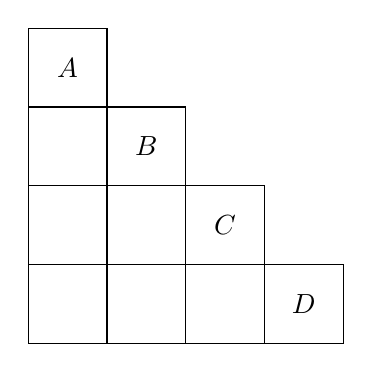
\begin{tikzpicture}
			\foreach \x in {0 ,..., 3}{
				\foreach \y in {0,..., \numexpr3 - \x\relax}
				{\draw (\x, \y) rectangle ++(1, 1);}
			}
			\foreach \x/\g/\i in {0/3/A, 1/2/B, 2/1/C, 3/0/D}
			\draw (\x + 0.5, \g + 0.5)node{$\mathbb{\i}$};
		\end{tikzpicture}
	\end{center}
	\shortans{$6118$}
	\loigiai{
		Gọi $x_1$, $x_2$, $x_3$, $x_4$ lần lượt là các số thuộc các ô A, B, C, D. \\
		Ta có: $x_4 = x_1 + 3d$, với $d$ là công sai của cấp số cộng. \\
		Khi đó, $x_1 + 3d \le 26$ và $x_1 \ge 1 \Rightarrow 3d \le 25 \Rightarrow d \le 8$. \\
		Lại có: $x_4 - x_3 = d \ge 4 \Rightarrow 4 \le d \le 8$ hay $d \in \left\{4; 5; 6; 7; 8\right\}$. \\
		Với $d = 4$, $x_4 = x_1 + 12 \le 26 \Rightarrow 1 \le x_1 \le 14$ nên có $14$ cách chọn $x_1$. \\
		Lần lượt có $\mathrm{C}_3^1$ cách chọn $1$ số đứng trước $x_2$, $\mathrm{C}_3^2$ cách chọn $2$ số đứng trước $x_3$ và $\mathrm{C}_3^3$ cách chọn $3$ số đứng trước $x_4$. \\
		Do đó, trường hợp này có $14{\mathrm{C}_3^1}{\mathrm{C}_3^2}{\mathrm{C}_3^3} = 126$ (cách). \\
		Tổng quát hóa, số cách chọn thỏa mãn là $$T = \displaystyle\sum\limits_{d = 4}^8{\left(26 - 3d\right){\mathrm{C}_{d - 1}^1}{\mathrm{C}_{d - 1}^2}{\mathrm{C}_{d - 1}^3}} = 24472.$$
		Vậy $\dfrac{T}{4} = \dfrac{24472}{4} = 6118$.
	}
\end{ex}

%TN3-03
\begin{ex} %[Thi thử THPT, Nguyễn Văn Trỗi - Hà Tĩnh, 2025 - 2026] %[2D1C3-6]
	Một doanh nghiệp dự định sản xuất không quá $400$ sản phẩm. Nếu doanh nghiệp sản xuất $x$ sản phẩm $\left(1 \le x \le 400\right)$ thì doanh thu nhận được khi bán hết số sản phẩm là $F\left(x\right) = x^3 - 1999x^2 + 1001000x + 250000$ (đồng). Trong đó, chi phí vận hành máy móc cho mỗi sản phẩm là $G\left(x\right) = \dfrac{100000x}{\dfrac{3}{2}x + 1}$ (đồng). Tổng chi phí mua nguyên vật liệu là $H\left(x\right) = 2x^3 + 100000x - 50000$ (đồng), nhưng do doanh nghiệp mua với số lượng lớn nên được ưu đãi giảm $1\%$ cho $200$ sản phẩm đầu tiên và giảm $2\%$ cho các sản phẩm tiếp theo. Doanh nghiệp cần sản xuất bao nhiêu sản phẩm để lợi nhuận thu được là lớn nhất?
	\shortans{$253$}
	\loigiai{
		Doanh thu: $F\left(x\right) = x^3 - 1999x^2 + 1001000x + 250000$ (đồng). \\
		Tổng chi phí vận hành: $xG\left(x\right) = \dfrac{100000x^2}{\dfrac{3}{2}x + 1}$ (đồng). \\
		Tổng chi phí mua nguyên vật liệu: $H\left(x\right) = 2x^3 + 100000x - 50000$ (đồng). \\
		Lợi nhuận khi sản xuất không quá $200$ sản phẩm $\left(1 \le x <\le 200\right)$ là $$L\left(x\right) = F\left(x\right) - xG\left(x\right) - 99\% H\left(x\right).$$
		Ta tìm được $L_{\max} = 80262059{,}41$ (đồng) tại $x = 183$ (sản phẩm). \\
		Lợi nhuận khi sản xuất từ $200$ sản phẩm trở lên $\left(200 < x \le 400\right)$ là $$L\left(x\right) = F\left(x\right) - xG\left(x\right) - 99\% H\left(200\right) - 98\% H\left(x - 200\right).$$
		Ta tìm được $L_{\max} = 83893648{,}05$ (đồng) tại $x = 253$ (sản phẩm). \\
		Vậy doanh nghiệp thu được lợi nhuận tối đa khi sản xuất $253$ sản phẩm.
	}
\end{ex}

%TN3-04
\begin{ex} %[Thi thử THPT, Nguyễn Văn Trỗi - Hà Tĩnh, 2025 - 2026] %[2D4V3-5]
	Nghề làm thùng gỗ sồi đựng rượu vang (đặc biệt là chuẩn thùng Barrique của vùng Bordeaux, Pháp) đòi hỏi sự tỉ mỉ và độ chính xác rất cao. Những chiếc thùng này không có dạng hình trụ thẳng đứng mà phình ra ở giữa. Thiết kế này giúp thợ ủ rượu dễ dàng lăn thùng và cặn rượu được gom lại ở phần rốn bụng. Theo tiêu chuẩn sản xuất, đường viền dọc thân thùng cong dạng một cung parabol.
	\begin{center}
		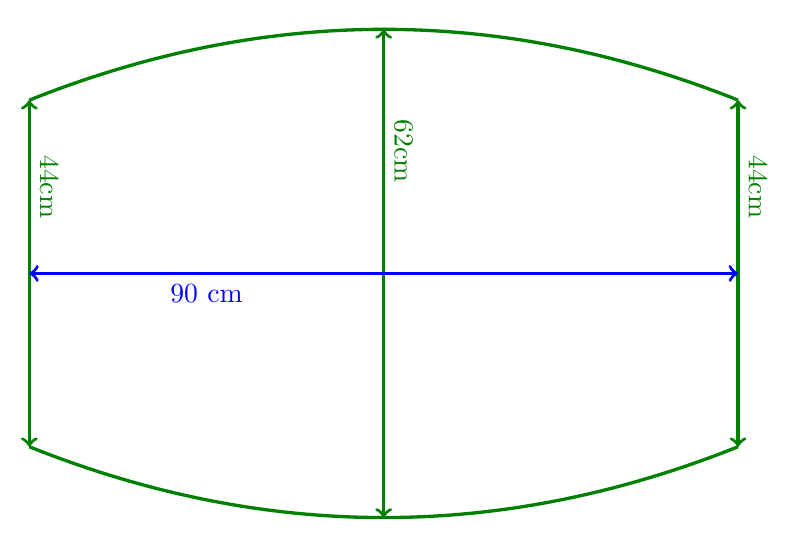
\begin{tikzpicture}[scale = .1]
			\def\hsf(#1){-4/900*(#1)^2 + 31} \def\hsg(#1){4/900*(#1)^2 - 31}
			\def\ca{-45} \def\cb{45}
			\draw[smooth, very thick, green!50!black] plot[domain = \ca:\cb, samples = 100] (\x, {\hsf(\x)});
			\draw[smooth, very thick, green!50!black] plot[domain = \ca:\cb, samples = 100] (\x, {\hsg(\x)});
			\foreach \i/\g in {\ca/44, \cb/44, 0/62}
			\draw[<->, very thick, green!50!black] (\i, {\hsf(\i)})--(\i, {\hsg(\i)})node[pos = .25, above, sloped]{\g cm};
			\draw[<->, very thick, blue] (\ca, 0)--(\cb, 0)node[pos = .25, below]{$90$ cm};
		\end{tikzpicture}
	\end{center}
	Một xưởng gỗ chuẩn bị xuất xưởng một chiếc thùng có các thông số kỹ thuật được đo đạc cẩn thận. Nhiệm vụ đặt ra là phải tính toán dung tích thực tế của chiếc thùng này để dán nhãn chính xác trước khi đưa vào hầm ủ. Biết rằng thùng rượu vang có chiều cao $90$ cm . Đường kính lớn nhất ở phần bụng thùng là $62$ cm , trong khi đường kính ở hai mặt đáy của thùng là bằng nhau và bằng $44$ cm . Hỏi thể tích của chiếc thùng đó bằng bao nhiêu lít (làm tròn kết quả đến hàng đơn vị).
	\shortans{$224$}
	\loigiai{
		\begin{center}
			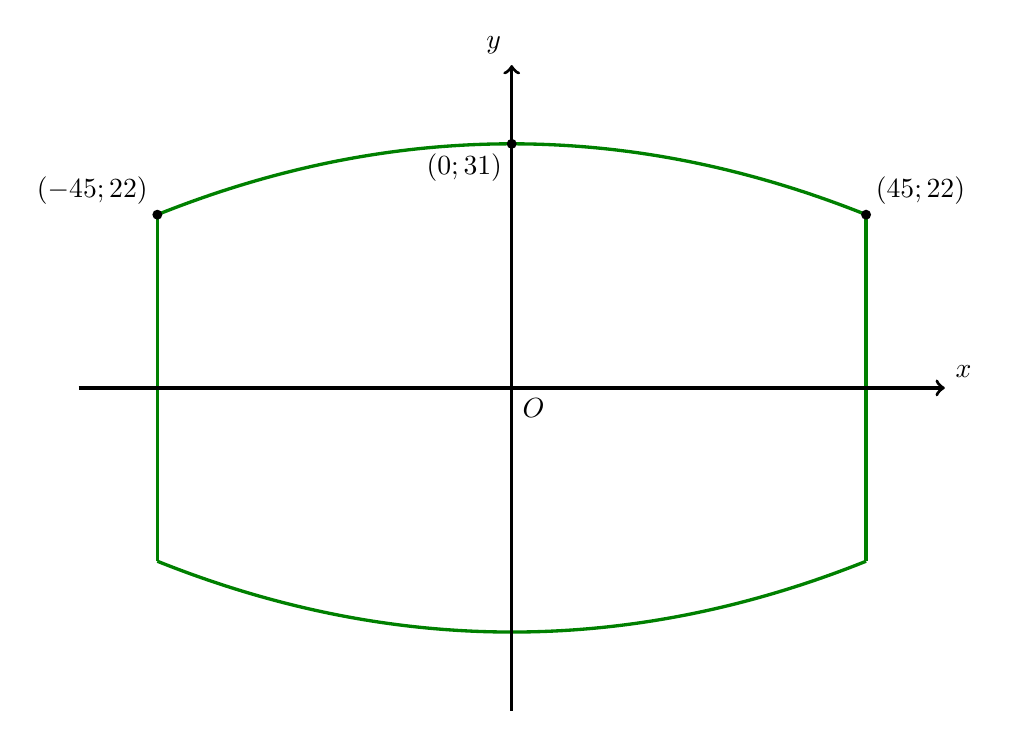
\begin{tikzpicture}[scale = .1]
				\def\hsf(#1){-4/900*(#1)^2 + 31} \def\hsg(#1){4/900*(#1)^2 - 31}
				\def\ca{-45} \def\cb{45}
				\draw[smooth, very thick, green!50!black] plot[domain = \ca:\cb, samples = 100] (\x, {\hsf(\x)});
				\draw[smooth, very thick, green!50!black] plot[domain = \ca:\cb, samples = 100] (\x, {\hsg(\x)});
				\foreach \i/\g in {\ca/44, \cb/44, 0/62}
				\draw[very thick, green!50!black] (\i, {\hsf(\i)})--(\i, {\hsg(\i)});
				\draw[very thick, blue] (\ca, 0)--(\cb, 0);
				\draw[->, very thick] (-55, 0)--(0, 0)node[below right]{$O$}--(55, 0)node[above right]{$x$};
				\draw[->, very thick] (0, -41)--(0, 41)node[above left]{$y$};
				\fill (-45, 22) circle (18pt) node[above left]{$\left(-45; 22\right)$} (0, 31) circle (18pt) node[below left]{$\left(0; 31\right)$} (45, 22) circle (18pt) node[above right]{$\left(45; 22\right)$};
			\end{tikzpicture}
		\end{center}
		Gắn hệ trục $Oxy$ như hình trên. Giả sử đường viền dọc thân thùng là parabol $\left(P\right) \colon y = ax^2 + bx + c\; \left(a \ne 0\right)$. \\
		Khi đó, thể tích chiếc thùng là thể tích khối tròn xoay khi quay hình phẳng giới hạn bởi parabol $\left(P\right)$, trục hoành và hai đường thẳng $x = -45$, $x = 45$ quanh trục hoành. \\
		Do $\left(P\right)$ có đỉnh $\left(0; 31\right)$ và đi qua điểm $\left(45; 22\right)$ nên $\heva{
			& c = 31 \\
			& -\dfrac{b}{2a} = 0 \\
			& a \cdot 45^2 + b \cdot 45 + c = 22} \Leftrightarrow \heva{
			& c = 31 \\
			& b = 0 \\
			& a = -\dfrac{1}{225}}$. \\
		Vậy $\left(P\right) \colon y = -\dfrac{1}{225}x^2 + 31 \Rightarrow V = \pi\displaystyle\int\limits_{-45}^{45}{\left(-\dfrac{1}{225}x^2 + 31\right)^2}{\mathrm{\, d}}x = 71208\pi = 223706{,}5297$ (cm$^3$), xấp xỉ $224$ lít.
	}
\end{ex}

%TN3-05
\begin{ex} %[Thi thử THPT, Nguyễn Văn Trỗi - Hà Tĩnh, 2025 - 2026] %[1H8V7-4]
	Cho khối lăng trụ $ABC.A'B'C'$ có đáy là tam giác đều cạnh bằng $5$. Hình chiếu vuông góc của điểm $A'$ lên mặt phẳng $\left(ABC\right)$ trùng với trọng tâm $G$ của tam giác $ABC$. Biết khoảng cách giữa hai đường thẳng $AA'$ và $BC$ bằng $\dfrac{15}{4}$. Tính thể tích của khối lăng trụ đã cho (làm tròn kết quả đến hàng đơn vị).
	\shortans{$54$}
	\loigiai{
		\immini{Gọi $M$ là trung điểm $BC$, kẻ $MK \perp AA'$. \\
			Khi đó, $\heva{
				& BC \perp AM \\
				& BC \perp A'G} \Rightarrow BC \perp \left(AA'G\right) \Rightarrow BC \perp MK$. \\
			Do đó, $\mathrm{d}\left(AA', BC\right) = MK = \dfrac{15}{4}$. \\
			Ta có: $AG = \dfrac{2}{3}AM = \dfrac{2}{3} \cdot \dfrac{5\sqrt 3}{2} = \dfrac{5\sqrt 3}{3}$; \\
			$AK = \sqrt{AM^2 - MK^2} = \sqrt{\left(\dfrac{5\sqrt 3}{2}\right)^2 - \left(\dfrac{15}{4}\right)^2} = \dfrac{5\sqrt 3}{4}$. \\
			Dễ thấy, $\triangle AA'G \sim \triangle AMK \Rightarrow \dfrac{A'G}{MK} = \dfrac{AG}{AK}$ \\
			$\Rightarrow \dfrac{A'G}{\dfrac{15}{4}} = \dfrac{\dfrac{5\sqrt 3}{3}}{\dfrac{5\sqrt 3}{4}} \Rightarrow A'G = 5$. \\
			Vậy $V_{ABC.A'B'C'} = A'G \cdot S_{ABC} = 5 \cdot\dfrac{5^2\sqrt 3}{4} = \dfrac{125\sqrt 3}{4} \approx 54$.}
		{\begin{tikzpicture}[scale = .75]
				\path
				(0:0) coordinate (A)
				++(-40:3) coordinate (B)
				(A)++(0:6) coordinate (C)
				%\foreach \x in {A, B, C}{(\x)++(90:6) coordinate(\x')}
				($(B)!.5!(C)$) coordinate (M)
				($(A)!2/3!(M)$) coordinate (G)
				++(90:6) coordinate (A')
				++(-40:3) coordinate (B')
				(A')++(0:6) coordinate (C')
				($(A)!2/5!(A')$) coordinate (K) 
				pic[draw, angle radius = 3mm]{right angle = A--M--C}
				pic[draw, angle radius = 3mm]{right angle = A--K--M}
				pic[draw, angle radius = 3mm]{right angle = A'--G--A};
				\draw[dashed, thick] (A)--(C) (A)--(M)
				(A')--(G) (A')--(M) (M)--(K);
				\draw[thick] (A)--(B)node[pos = .5, below]{$5$} (B)--(C) (A')--(B') (B')--(C') (C')--(A')
				(A)--(A') (B)--(B') (C)--(C');
				\foreach \x/\g in {A/-135, B/-90, C/0, A'/135, B'/-15, C'/45, G/-135, M/-15, K/135}
				\draw[fill] (\x) circle (.03) + (\g:.4) node{$\x$};
		\end{tikzpicture}}
	}
\end{ex}

%TN3-06
\begin{ex} %[Thi thử THPT, Nguyễn Văn Trỗi - Hà Tĩnh, 2025 - 2026] %[0D2V2-3]
	Một học sinh mở tiệm online chuyên kinh doanh hai mặt hàng: Gấu bông len cỡ lớn và Túi len (phụ kiện). Để móc hoàn thiện một chiếc Gấu bông len cỡ lớn, bạn ấy cần $6$ giờ. Để móc hoàn thiện một chiếc Túi len, bạn ấy cần $4$ giờ. Vì bận lịch học, mỗi tuần bạn ấy chỉ có tối đa $36$ giờ để làm đồ len. Để đảm bảo gian hàng đa dạng, bạn ấy đặt ra quy tắc: số lượng Túi len làm ra không được nhiều hơn số Gấu bông len quá $1$ cái. Đồng thời, do nguồn nguyên liệu len nhập về có hạn, tổng số sản phẩm cả hai loại bạn ấy có thể làm trong một tuần tối đa là $7$ cái. Biết rằng mỗi chiếc Gấu bông len mang lại lợi nhuận $180$ nghìn đồng, và mỗi chiếc Túi len mang lại lợi nhuận $140$ nghìn đồng. Gọi $x$ và $y$ lần lượt là số Túi len và số Gấu bông len mà bạn học sinh làm được trong một tuần ($x, y \ge 0$ và là số nguyên). Số tiền lãi lớn nhất mà bạn học sinh này có thể thu được trong một tuần là bao nhiêu nghìn đồng?
	\shortans{$1140$}
	\loigiai{
		Bài toán đưa về tìm $x, y$ là nghiệm của hệ bất phương trình $\heva{
			& 4x + 6y \le 36 \\
			& x - y \le 1 \\
			& x + y \le 7 \\
			& x, y \ge 0}$ sao cho $P\left(x, y\right) = 140x + 180y$ có giá trị lớn nhất. \\
		\begin{center}
			\begin{tikzpicture}[scale = 1, >= stealth]
				% Trục toạ độ
				\draw[->] (0, 0)node[below left]{$O$}--(10, 0)node[below]{$x$};
				\draw[->] (0, 0)--(0, 10)node[left]{$y$};
				% Các bất phương trình
				\draw[thick, blue] (0, 6)--(9, 0)node[above right, blue]{$4x + 6y = 36$};
				\draw[thick, red] (1, 0)--(10, 9)node[above, red]{$x - y = 1$};
				\draw[thick, teal] (0, 7)node[above right, teal]{$x + y = 7$}--(7, 0);
				% Gạch phần ngoài miền nghiệm
				\path[pattern = north east lines, pattern color = blue!50, opacity = 0.5] (0, 6)--(0, 10)--(10, 10)--(10, 0)--(9, 0)--cycle;
				\path[pattern = north west lines, pattern color = red!50, opacity = 0.5] (1, 0)--(10, 0)--(10, 9)--cycle;
				\path[pattern = north west lines, pattern color = teal!50, opacity = 0.5] (0, 7)--(0, 10)--(10, 10)--(10, 0)--(7, 0)--cycle;
				% Miền nghiệm khả thi
				\fill[yellow, opacity = 0.5] (0, 6)--(3, 4)-- (4, 3)--(1, 0)--(0, 0)--cycle;
				% Đánh dấu các đỉnh
				\node[left] at (0, 6) {$A\left(0; 6\right)$};
				\node[left] at (3, 4) {$B\left(3; 4\right)$};
				\node[left] at (4, 3) {$C\left(4; 3\right)$};
				\node[below] at (1, 0) {$D\left(1; 0\right)$};
				\fill[black] (0, 6) circle (2pt) (3, 4) circle (2pt) (4, 3) circle (2pt) (1, 0) circle (2pt);
			\end{tikzpicture}
		\end{center}
		Miền nghiệm của hệ bất phương trình là miền đa giác $OABCD$ như hình trên với $A\left({0; 6}\right)$, $B\left({3; 4}\right)$, $C\left({4; 3}\right)$ và $D\left({1; 0}\right)$. \\
		Biểu thức $P\left({x, y}\right) = 140x + 180y$ đạt giá trị lớn nhất tại một trong các đỉnh này:
		\begin{enumEX}[\small $\bullet$]{2}
			\item ${P_A} = 140 \cdot 0 + 180 \cdot 6 = 1080$;
			\item ${P_B} = 140 \cdot 3 + 180 \cdot 4 = 1140$;
			\item ${P_C} = 140 \cdot 4 + 180 \cdot 3 = 1100$;
			\item ${P_D} = 140 \cdot 1 + 180 \cdot 0 = 140$.
		\end{enumEX}
		Vậy số tiền lãi lớn nhất có thể thu được là $1140$ nghìn đồng khi làm $3$ Túi len và $4$ Gấu bông len.
	}
\end{ex}
\Closesolutionfile{ans}

\indapan{6}{ans/ans-26-2--SoGD-L1-LC}
\indapan{4}{ans/ans-26-2--SoGD-L1-DS}
\indapan{6}{ans/ans-26-2--SoGD-L1-KQ}